\documentclass[../paper.tex]{subfiles}

\begin{document}
  \subsection{Technology Stack}

  The goal of this project in terms of the implementation was to
  build a web application that is easily embeddable into a mobile application.
  For this reason we decided on going for a lean front end without too many
  unnecessary dependencies to keep it responsive. Among the key dependencies that
  are necessary is D3.js, a JavaScript library for manipulating documents based
  on data \cite{d3}. D3 fits the requirements of simple interoperability between
  data and visualisation by manipulating the DOM perfectly.

  Naturally a front end for the purpose of this application is not of much use
  without data and therefore a database is required. Given that the
  visualisation is build around a semantic knowledge graph, a graph database is
  a necessity.

  A great fit in this regard is RDF4J. RDF4J, a native triple
  store, offers the ability to query the knowledge graph using SPARQL. The
  database has also support for all mainstream RDF file formats \cite{rdf4j}.
  RDF4J is an open-source project under the umbrella of the Eclipse Foundation
  which indicates it is trusted by a big community.

  Another option is GraphDB \cite{graphdb}, a proprietary graph database developed by Ontotext.
  It offers multiple APIs for querying the database, including RDF4J and SPARQL,
  among other things. Ontotext offers a free version of GraphDB, however when
  we evaluated it for development purposes, it was not really suitable for a
  fully automatic development experience given that the free version needs to
  be downloaded manually while Ontotext offers pre-built Docker images for
  their Standard and Enterprise offerings.

  Since the CampaNeo project already had a pre-existing GraphDB database, we
  still decided on using GraphDB. The main focus of this project is the
  visualisation, so as long as we could retrieve the data from the database
  this did not pose a problem for our purposes. The multiple APIs offered by
  GraphDB allowed us to use a vendor-agnostic JavaScript framework for
  creating SPARQL queries.

  A simple use case would be a user starting the application, which initializes
  the D3 frontend web application, which in turn queries data from the database
  to visualize the consent page as shown in \cref{fig:prototype}.

  \subsection{Architecture}

  Shown in \cref{fig:architecture} is an overview of the technical architecture
  for the implementation of the data visualization:

  \begin{figure}
    \centering
    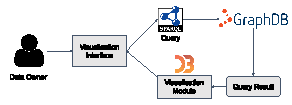
\includegraphics[width=\linewidth]{architecture.pdf}
    \caption{Technical Architecture}
    \label{fig:architecture}
  \end{figure}

  On the left side of \cref{fig:architecture} we see the application user, i.e.
  the data owner. The data owner interacts only with the front end part of the
  application, which we call the “Visualisation Interface”.

  On first load or whenever the user interacts with the interface in such a way
  that the underlying data needs to be updated, we send a SPARQL query to the
  GraphDB database. Once the result of this query is retrieved, it is passed to
  the “Visualisation Module”. This module processes the data depending on
  whether it will be displayed in the overview visualisation or the detailed
  time series visualisation and produces the corresponding visualisation
  using \texttt{D3.js} accordingly.

  Depending on the query, we get a lot of data in return, as the database
  will return a value for each data-package, that was sent. The so called
  "Visualisation Module" groups those together, creating a single visible
  node for each category of data. These categories are predefined in the
  ontology and represent thing like coordinates, longitude and latitude, or
  fuel consumption. The module then creates connections between the data packages
  and the third party companies receiving them.

  After the visualization is created for the received data, the “Visualisation Module”
  updates the currently displayed graph.

  % TODO: Explain the “Visualisation Module” in more detail. Maybe add a second
  %       diagram showing the inner workings of the module.

  …
\end{document}
